\documentclass[]{artikel3}
\usepackage[]{amsmath}
\usepackage{listings}
\usepackage{xcolor}
\usepackage{graphicx}
\usepackage{siunitx}

\definecolor{codegreen}{rgb}{0,0.6,0}
\definecolor{codegray}{rgb}{0.5,0.5,0.5}
\definecolor{codepurple}{rgb}{0.58,0,0.82}
\definecolor{backcolour}{rgb}{0.95,0.95,0.92}

\lstdefinestyle{mystyle}{
    backgroundcolor=\color{backcolour},
    commentstyle=\color{codegreen},
    keywordstyle=\color{magenta},
    numberstyle=\tiny\color{codegray},
    stringstyle=\color{codepurple},
    basicstyle=\ttfamily\footnotesize,
    breakatwhitespace=false,
    breaklines=true,
    captionpos=b,
    keepspaces=true,
    numbers=left,
    numbersep=5pt,
    showspaces=false,
    showstringspaces=false,
    showtabs=false,
    tabsize=2
}

\lstset{style=mystyle, language=Octave}

\title{From backscatter to suspended sediment concentrations}
\author{Bart Vermeulen}

\begin{document}
\maketitle

\section{Introduction}
In this document first a theoretical overview is given of different methods to compute sediment concentration from backscatter strength of ADCPs. Subsequently, a step-by-step guide explains how to perform the calibration using the adcptools.

\section{Calibration methods}
All calibration require water samples to be collected from which suspended sediment concentration is obtained, usually through filtration of the samples. Subsequently a relation is sought between backscatter strength and concentration.
A simple straightforward method is the power law method (e.g. Hoitink and Hoekstra, 2005). This method, however, does not take into account the effect of attenuation.  Another method by Sassi et al. 2012, assumes a constant specific attenuation and calibrates an attenuation and a backscatter constant. It is recommended to first use the simple power law method and if needed the more complex constant specific attenuation methods.
\subsection{The power law method}
The power law method assumes a relation between suspended sediment concentration $M$ and the backscatter strength $S_v$:
\begin{equation}
  \frac{M}{M_0}=10^{aS_v+b}
\end{equation}
With $M_0$ equal to \SI{1}{\milli\g\per\liter}.
\subsection{The constant specific attenuation method}

\subsubsection{Introduction}
In order to obtain mass concentrations from ADCP backscatter signal we need to perform a calibration. The method propose by Sassi et al., 2012 assumes a constant particle size distribution of sediments and a constant sediment induced attenuation between two consecutive measurements.

\subsubsection{The calibration method in a nutshell}
The method essentially consists of calibrating two parameters:
\begin{itemize}
  \item $b$ which expresses the relation between sediment backscatter and mass concentration in absence of attenuation
  \item $\xi_s$ attenuation per unit concentration (specific attenuation)
\end{itemize}
The first parameter $b$ requires a sample collected very close to the ADCP transducer (but outside of the blanking distance), such that we can assume the effect of attenuation to be negligible.
To estimate the second parameter $\xi_s$ another sample can be collected at a larger depth. This sample should preferably be near the last cell of the ADCP. More samples can be collected at different depths to estimate depth variations in $\xi_s$.

Next to these basic parameters, there are a number of additional parameters that can be calibrated:
\begin{itemize}
  \item The RSSI scale factor $K_c$ (dB/count) and the calibration coefficient $C$ are both instrument specific constants that can be calibrated when water samples are available at the start of the ADCP measuring range and with known grain size distribution.
  \item The density of the backscattered particles $\rho_s$ can be calibrated when both mass concentrations (e.g. from filtration) and volume concentration (e.g. from Malvern or LISST) are available
\end{itemize}

\section{Minimum required inputs}
To estimate parameters $b$ and $\xi_s$ we will need:
\begin{itemize}
  \item Water samples near the transducer, but far enough to be in the detection range of the ADCP (outside the blanking distance)
  \item Water samples deeper in the water column.
    \begin{itemize}
      \item At least one or more at the end of the ADCP measuring range.
      \item Optionally samples at more depths if variations in $\xi_s$ are expected over depth (e.g. changing grain size distribution)
    \end{itemize}
  \item Exact depth the samples were taken
  \item Time the samples were taken
  \item ADCP echo intensity values from the ADCP collected at the time the sample was taken (2-3 minutes of data are recommended)
  \item Transducer characteristics
    \begin{itemize}
      \item Operating frequency
      \item Diameter
      \item RSSI scale factor $K_c$ (dB/count, ADCP characteristic which can be obtained from the manufacturer, calibrated in a lab with a hydrophone or estimated if grain size distributions have been determined.)
      \item RSSI in a bucket $E_r$ (counts, background noise, see PT3 command on RDI ADCPs)
      \item Calibration coeff $C$ (dB, instrument specific constant, can be obtained from manufacturer or estimated if grain size distributions have been determined.)
    \end{itemize}
  \item Water characteristics
    \begin{itemize}
      \item Temperature
      \item Salinity (For stratified conditions CTD data are needed)
    \end{itemize}
  \item Depth of the ADCP transducer (insteekdiepte)
\end{itemize}

\section{Computations}
The computations will be performed in the following order:
\begin{enumerate}
  \item Compute $\rho_s$, if volume and mass concentration are available for sample
  \item Calibrate $K_c$ and $C$ if GSD is available for samples collected near the transducer
  \item Calibrate $b$ and $\xi_s$ from mass concentration samples
  \item Compute mass concentration profiles for volume backscatter strength
\end{enumerate}

\subsection{Calibration of $\rho_s$ (optional)}
$\rho_s$ is easily estimated when mass concetration $M_\text{s}$ and volume concentration $C$ are available:
\begin{equation}
  \rho_s=\dfrac{M_s}{C}
\end{equation}
Specifying the \lstinline!volume_concentration! and \lstinline!mass_concentration! properties of the \lstinline!acoustics.WaterSample! class will automatically compute the density given in the \lstinline!sediment_density! property.
\subsection{Calibration of $K_c$ and $C$ (optional)}
The basis for this calibration is that we can compute the volume backscatter strength $S_v$ both from the GSD and sediment concentration and from the ADCP backscatter. Than we can estimate $K_c$ and $C$ as unknowns.
The first step is to estimate the $k_s^2$. This is based on the mean backscatter cross-section $\langle\sigma_{bs}\rangle$ that is computed from the form function and the GSD:
\begin{align*}
  S_v=&10\log_{10}(k_s^2M_s)\\
  k_s^2=&\dfrac{3}{16\pi\rho_s}\dfrac{\langle a_s^2 f^2 \rangle}{\langle a_s^2\rangle}\\
\end{align*}
In \texttt{adcptools} we will first need to create an \texttt{acoustics.PisontTransducer} object.
\begin{lstlisting}[language=Octave]
pt=acoustics.PistonTransducer;
\end{lstlisting}
Than we set the right frequency and transducer diameter:
\begin{lstlisting}[language=Octave]
pt.frequency=1228.8e3; %for a 1200 kHz ADCP
pt.radius=0.027; % radius of 2.7 cm
\end{lstlisting}
The \texttt{acoustics.PistonTransducer} object also contains a \texttt{Water} object that is used to compute the speed of sound in water given temparature, salinity and pH.

Now we can construct an \texttt{acoustics.GrainSizeDistribution} object and assign fractions and diameters:
\begin{lstlisting}
gs=1e-6*[0.01 0.011482 0.013183 0.015136 0.017378 0.019953 0.022909 0.026303 0.0302 0.034674 0.039811 0.045709 0.052481 0.060256 0.069183 0.079433 0.091201 0.104713 0.120226 0.138038 0.158489 0.18197 0.20893 0.239883 0.275423 0.316228 0.363078 0.416869 0.47863 0.549541 0.630957 0.724436 0.831764 0.954993 1.096478 1.258925 1.44544 1.659587 1.905461 2.187762 2.511886 2.884031 3.311311 3.801894 4.365158 5.011872 5.754399 6.606934 7.585776 8.709636 10 11.481536 13.182567 15.135612 17.378008 19.952623 22.908677 26.30268 30.199517 34.673685 39.810717 45.708819 52.480746 60.255959 69.183097 79.432823 91.201084 104.712855 120.226443 138.038426 158.489319 181.970086 208.929613 239.883292 275.42287 316.227766 363.078055 416.869383 478.630092 549.540874 630.957344 724.43596 831.763771 954.992586 1096.478196 1258.925412 1445.439771 1659.586907 1905.460718 2187.761624 2511.886432 2884.031503 3311.311215 3801.893963 4365.158322 5011.872336 5754.399373 6606.93448 7585.77575 8709.6359 10000];
fract=.01*[0 0 0 0 0 0 0 0 0 0 0 0 0 0 0 0 0 0 0 0 0 0 0 0 0 0 0 0.178333 0.301668 0.385886 0.445449 0.469272 0.467858 0.449735 0.42987 0.422813 0.441772 0.49676 0.595676 0.749952 0.974694 1.284648 1.689853 2.185246 2.760847 3.378964 4.007627 4.583791 5.068609 5.405399 5.574199 5.560831 5.378561 5.063955 4.655804 4.211591 3.768856 3.366553 3.018285 2.730382 2.494196 2.29615 2.120405 1.951593 1.781102 1.601525 1.414943 1.222138 1.035633 0.861343 0.712813 0.587049 0.47997 0.380193 0.279534 0.188959 0.073695 0.01502 0 0 0 0 0 0 0 0 0 0 0 0 0 0 0 0 0 0 0 0 0 0];
gsd=acoustics.GrainSizeDistribution(gs,fract);
\end{lstlisting}
Now we can compute all kinds of acoustic characteristics of the sediment. A quick view can be obtined by running:
\begin{lstlisting}
gsd.plot_all(pt)
\end{lstlisting}
This will produce a figure similar to figure~\ref{fig:gsd}.
\begin{figure}[h]
  \centering
  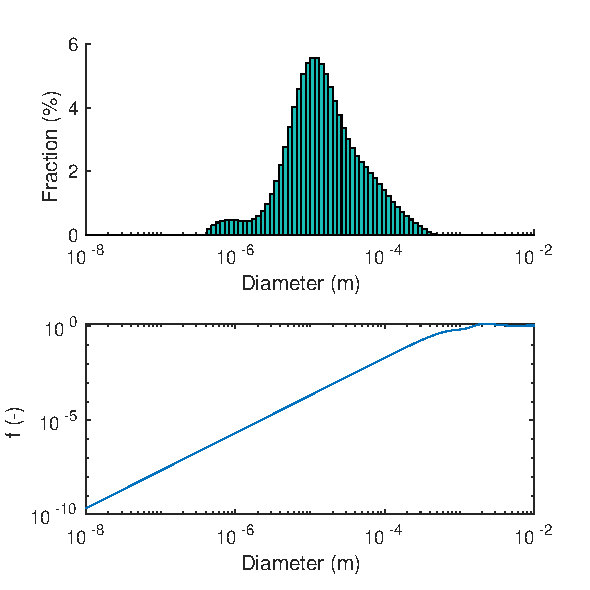
\includegraphics{gsd.pdf}
  \caption{Example of grain size distribution and the corresponding form function}
  \label{fig:gsd}
\end{figure}
The $k_s^2$ is now easily obtained as:
\begin{lstlisting}
ks2=gsd.ks_squared(pt, rhos);
\end{lstlisting}
Now that the $k_s^2$ is computed the $S_v$ is easily obtained having the sediment concentration.

\subsection{Calibration}
For the calibration we will need to first estimate the backscatter strength under the assumption that ther is no sediment attenuation $S_{v,\alpha_s=0}$:
\begin{align}
  S_{v,\alpha_s=0}= C + 10\log_{10}\dfrac{(T+273.16)R^2 \psi^2}{PL_\text{T}}  + 2\alpha_\text{w}R + 10\log10\left(10^{\frac{K_\text{c}E}{10}}-10^{\frac{K_\text{c}E_\text{r}}{10}}\right)
\end{align}
This computation can be performes with the \texttt{svADCP.m} script. This script requires as input the adcp structure (read by \texttt{readADCP.m}) and a \texttt{acoustics.PisontTransducer} object. Please note that this equation is the equation as proposed by Gostiaux and van Haren (2010), in which the last term differs from Deines (1999).

The following steps are all performed with the script \texttt{sassi\_inversion.m}.

\textbf{Part 1: estimate $b$}\\
Once this uncorrected backscatter strength is obtained, the first calibration step can be performed in which we try to estimate the parameter $b$ from equation 14 of Sassi et al.(2012):
\begin{align}
  K(R_\text{ref})=a\beta(\tilde{R}_\text{ref})^b
\end{align}
where $R_\text{ref}$ is the range where the water samples were collected, $K=\beta/M_\text{s}$, $\beta=10^{S_{\text{v,}\alpha_\text{s}=0}/10}$, $M_s$ is the measured sediment concentration, $a=1/[M_\text{s}]$ (i.e. the inverse of the sediment concentration unit). 

\textbf{Part 2: estimate $\xi_s$}\\
The last step of the calibration will yield $\xi_s$ using equation 15 from Sassi et al. (2012):
\begin{align}
  \gamma_e=\dfrac{\ln(10)}{5}\xi_s=\dfrac{K(R_1)-\dfrac{\beta(R_2)}{M_s(R_2)}}{\int_{R_1}^{R_2}\beta(r)\;\text{d}r}
\end{align}
For this step we will need to samples. The first can correspond with the sample used during the first calibration step, The second should preferably be near the end of the ADCP measuring range. This last step can be done with different combinations of samples to obtain $\xi_s$ varying over depth.


\subsection{Estimate sediment concentration}
The last step is to use the calibration to compute sediment concentration profiles for the measured ADCP data.
This is done by using equation 13 from Sassi et al. (2012):
\begin{align}
  M_s(R)=\dfrac{\beta(R)}{K(R_\text{ref})-\gamma_e\int_{R_\text{ref}}^R\beta(r)\;\text{d}r}
\end{align}
\end{document}
